\documentclass[11pt, oneside]{article}
\usepackage[margin=1in]{geometry}
\geometry{letterpaper}
\usepackage{graphicx}
\usepackage{amssymb}
\usepackage[parfill]{parskip}
\usepackage{amssymb}
\usepackage{amsmath}
\usepackage{listings}
\usepackage{color}
\usepackage{standalone}
\usepackage{gensymb}
\usepackage{tikz}
\usetikzlibrary{matrix,chains,positioning,decorations.pathreplacing,arrows}
\usepackage{wrapfig}
\usepackage{epstopdf}
\usepackage{float}

\graphicspath{ {code/images/} }

\def\layersep{2.5cm}

\sloppy
\definecolor{lightgray}{gray}{0.5}
\setlength{\parindent}{0pt}
\definecolor{dkgreen}{rgb}{0,0.6,0}
\definecolor{gray}{rgb}{0.5,0.5,0.5}
\definecolor{mauve}{rgb}{0.58,0,0.82}

\lstset{frame=tb,
  language=Matlab,
  aboveskip=3mm,
  belowskip=3mm,
  showstringspaces=false,
  columns=flexible,
  basicstyle={\small\ttfamily},
  numbers=none,
  numberstyle=\tiny\color{gray},
  keywordstyle=\color{blue},
  commentstyle=\color{dkgreen},
  stringstyle=\color{mauve},
  breaklines=true,
  breakatwhitespace=true,
  tabsize=3
}

\title{Neuro 120 Homework 4: Short and Long Term Memory}
\author{William Schmitt and Will Drew}
\date{Due: Thursday 15 November 2018}

\begin{document}
\maketitle

\section{Short Term Memory}

\subsection{RNN Dynamics with No Recurrent Connections}

\begin{figure}[ht!]
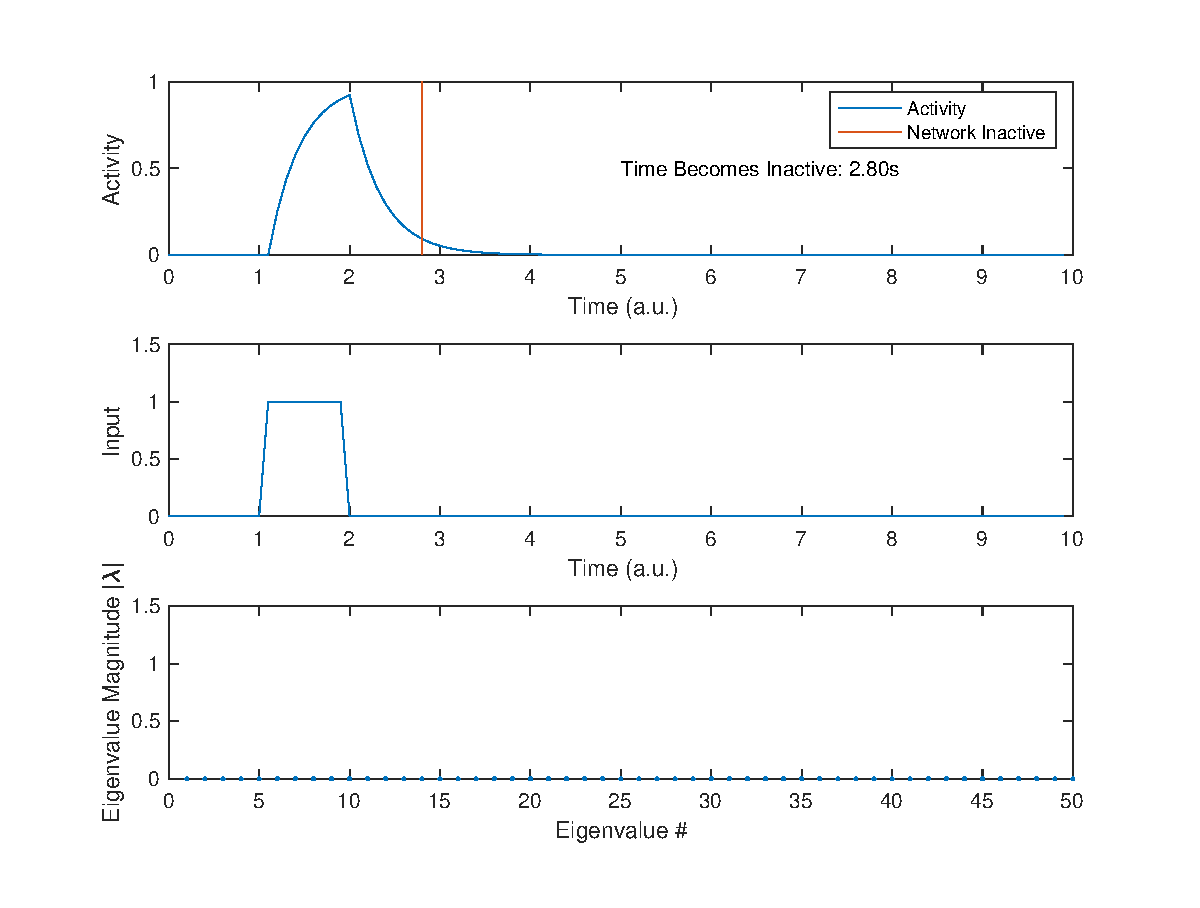
\includegraphics[width=1\textwidth]{RNNnoR.eps}
\caption{The dynamics of a RNN with no recurrent connections.}
\label{fig:RNNnoR}
\end{figure}

We build the RNN with the following code:
\lstinputlisting{code/shortterm_mem.m}
This code produces Figure \ref{fig:RNNnoR}, which we can see tells us that the activity in the network has died out at $t = 2.8$s.

\subsection{RNN with Autapses}

We comment out line 16 and uncomment line 18 and 19 of the code attached above to run the network as a set of autapses. Further, we run this three times, altering the weight scale in line 18 to be 0.9, 1, and 1.1. This produces Figures \ref{fig:RNN09}, \ref{fig:RNN10}, and \ref{fig:RNN11}.

In Figure \ref{fig:RNN09}, we see that activity in the network has not died out completely 9 seconds after the pulse, but it seems like if we expanded the time scale, the network activity would die out at around 12-14 seconds. \\
In Figure \ref{fig:RNN10}, we see that activity in the network remains stable after $t = 2$s.\\
In Figure \ref{fig:RNN11}, we see that activity in the network appears to diverge towards $+\infty$.

\begin{figure}[H]
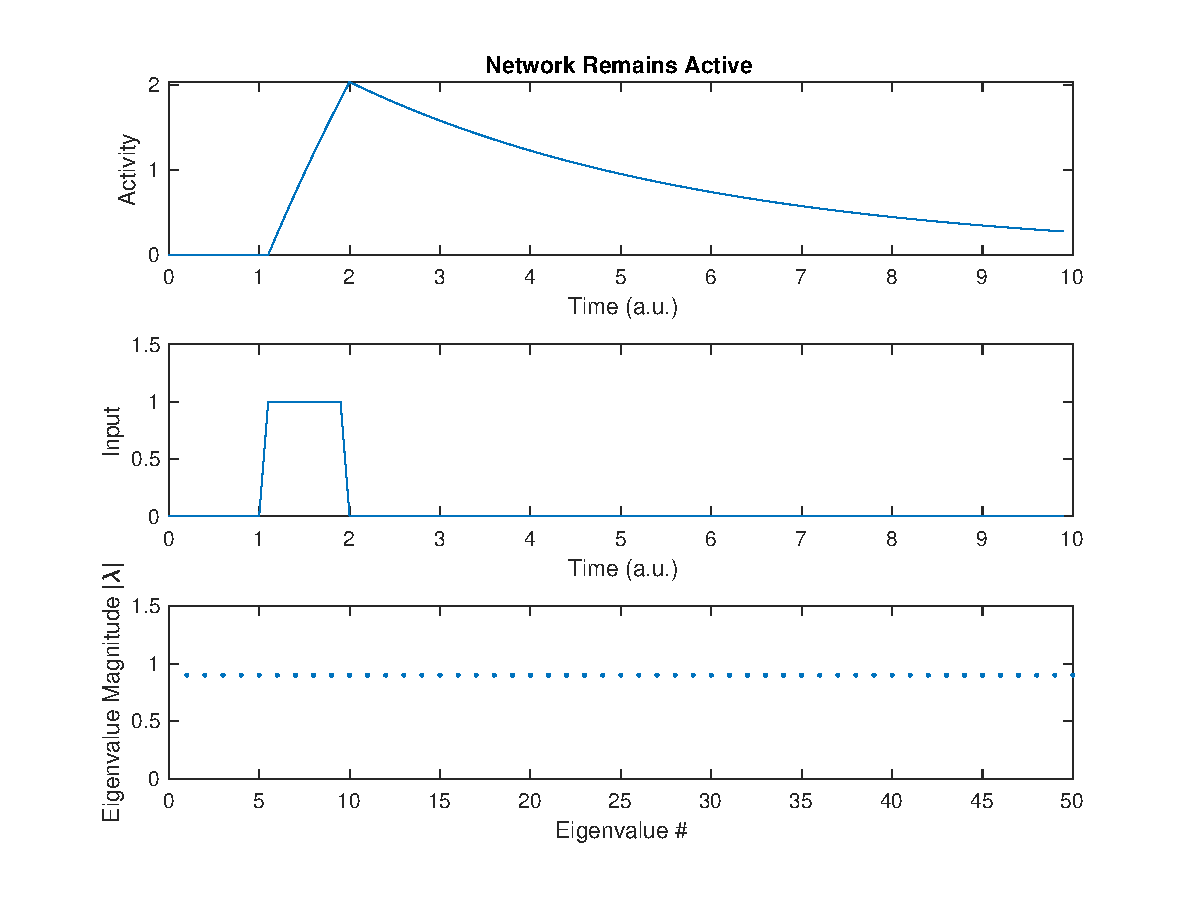
\includegraphics[width=1\textwidth]{RNN09.eps}
\caption{The dynamics of a RNN with autapses. $c = 0.9$}
\label{fig:RNN09}
\end{figure}

\begin{figure}[H]
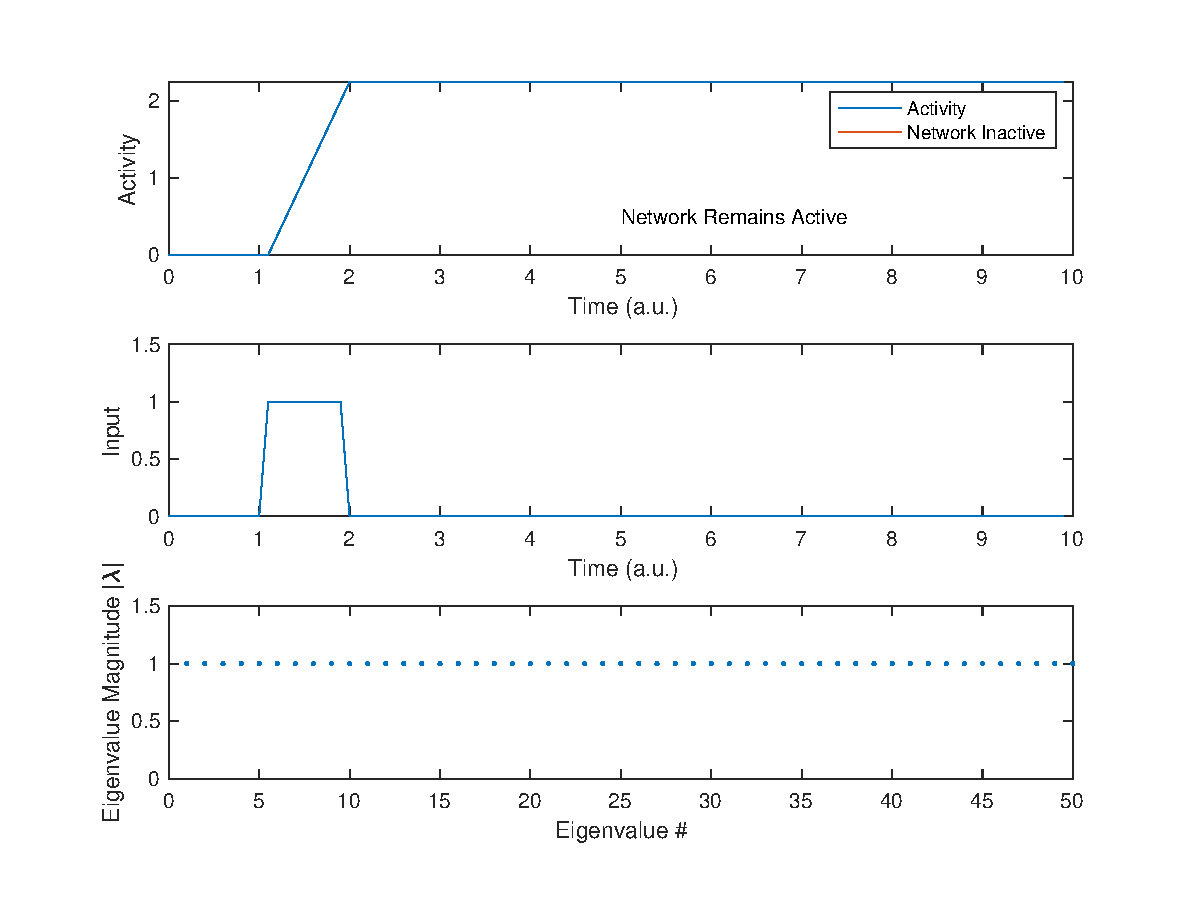
\includegraphics[width=1\textwidth]{RNN10.eps}
\caption{The dynamics of a RNN with autapses. $c = 1.0$}
\label{fig:RNN10}
\end{figure}

\begin{figure}[H]
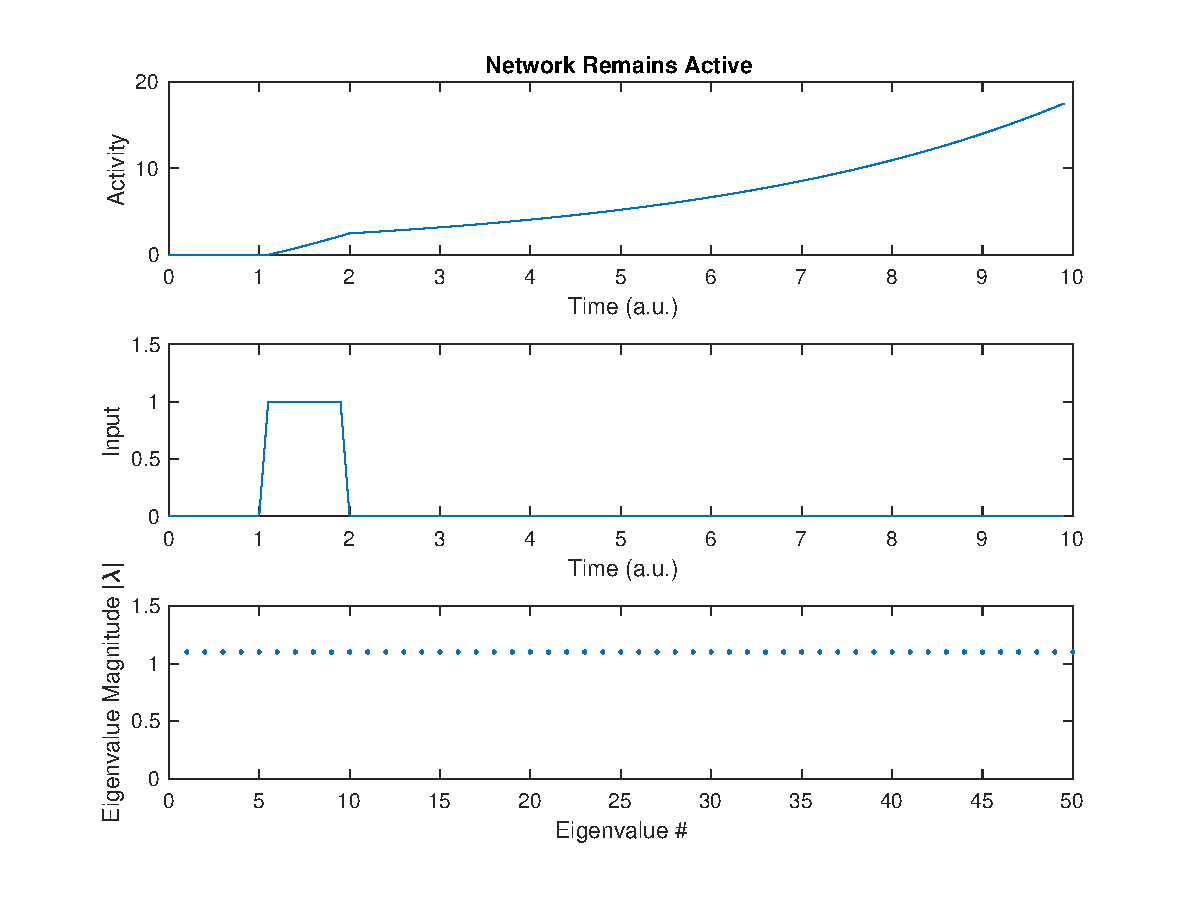
\includegraphics[width=1\textwidth]{RNN11.eps}
\caption{The dynamics of a RNN with autapses. $c = 1.1$}
\label{fig:RNN11}
\end{figure}

The magnitude of the eigenvalues of the recurrent matrix $W$ appear to be correlated with the weight scale $c$. In fact, they appear to have equal values!

We see that when the input is on, the activity increases as expected as $VI(t)$ adds to the rate of change of neuronal activity. When the input is off, that term disappears and we are left with $(c-1)r(t)$. When $c$ is less than 1 $(c=0.9)$, this term is negative, and neuronal activity decreases during this period towards 0. When $c = 1$, we see that this term is 0, indicating that there is no change in neuronal activity during this period. When $c$ is greater than 1 $(c=1.1)$, then this term is positive, indicating that neuronal activity should be increasing during this period.

Thus, the best choice of $c$ to stably store a memory would be $c=1$, as neuronal activity remains constant, neither dying out over time nor diverging towards infinity (brains crashing!).

\end{document}
